\documentclass[12pt]{article}
\usepackage[T2A]{fontenc}
\usepackage[utf8]{inputenc}
\usepackage[english,russian]{babel}
\usepackage{amssymb,amsmath,amsthm, mathtools}
\usepackage{subfigure}
\newcommand\independent{\protect\mathpalette{\protect\independenT}{\perp}}
\DeclareMathOperator{\trace}{trace}
\def\independenT#1#2{\mathrel{\rlap{$#1#2$}\mkern2mu{#1#2}}}


\newtheorem{note}{Замечание}
\newtheorem{theorem}{Теорема}
\newtheorem{dfn}{Определение}

\begin{document}

\section{Математическое описание MRF} 
Марковское случайное поле (MRF) это графическая модель совместного распределения нескольких случайных величин. Иными словами, это неориентированный граф $G = (\mathcal{N}, \mathcal{E})$, где множество вершин $\mathcal{N}$ -- это множество случайных величин. 
Множество случайных величин связанных с множеством вершин $S$ будем обозначать $X_S$. Ребра $\mathcal{E}$ указывают на условную независимость: пусть $A, B$ и $C$ --- непересекающиеся подмножества вершин. Говорят, что $X_A$ условно независимо с $X_B$ при условии $X_C$, если не существует путей из вершины множества $A$ в вершину множества $B$, которая не проходит через $C$ (рисунок \ref{fig:mrf} (a)). Будем обозначать условную независимость как $X_A \independent X_B \mid X_C$.

Будем обозначать всех соседей вершины $n$ за $N_n$: 
\begin{equation*}
N_n = \{ m \in \mathcal{N} \mid (m, n) \in \mathcal{E}\}.
\end{equation*}
Имеет место Марковское свойство (отсюда и название):
\begin{equation*}
P(X_n \mid X_\mathcal{N} - X_n) = P(X_n \mid X_{N_n})
\end{equation*}

На рисунке \ref{fig:example} при условии серых вершин черная условно независима с остальными.

\begin{figure}[hhh]
\centering
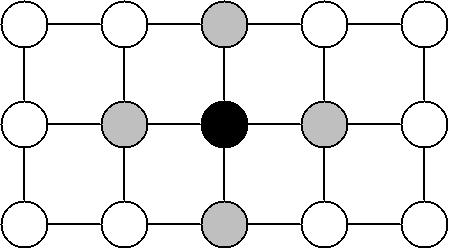
\includegraphics[width=.5\linewidth]{figures/blanket.jpg}
\label{fig:example}
\caption{Пример графа для пиксельного изображения}
\end{figure}

Далее, реализацию Марковского случайного поля будем обозначать $x$ с индексом, соответсвующем подмножеству вершин.

\begin{dfn}
Кликой будем называть полный подграф исходного графа. Клика называется максимальной, если при добавлении новой вершины в нее, подраф перестает быть полным.
\end{dfn}
На рисунке \ref{fig:mrf} (b) максимальная клика обозначена синим цветом.

Чтобы определенить совместное распредедление MRF нам понадобится следущая теорема:
\begin{theorem}[Хаммерсли-Клиффорд]
Положительное распределение $p(y) > 0$ удовлетворяет свойствам условной независимости неориентированного графа $G$ тогда и только тогда, когда $p$ можеть быть представлено в виде:
\begin{equation}
p(x) = \frac{1}{Z} \prod\limits_{C \in \mathcal{C}} \psi_C(x_C), 
\label{eqn:jointdens}
\end{equation}
где $Z  = \sum\limits_{x \in \mathcal{X}} \prod\limits_{C \in \mathcal{C}} \psi_C(x_C)$.
При этом $\mathcal{С}$ -- множество максимальных кликов.
\end{theorem}


Чаще всего $\psi_C(x_C) = exp(-V_C(x_C)/T)$ и тогда совместная плотность принимает вид:
\begin{equation}
p(x) = \frac{1}{Z} \exp\left(-\frac{1}{T} U(x)\right),   
\label{eqn:eng_function}
\end{equation}
$U(x) = \sum_{C \in \mathcal{C}}V_C(x_C)$ будем называть функцией энергии.
Теорема  Хаммерсли-Клиффорда утверждает, что любое совместное распределение может быть записано как произведение распределене Гиббса. Более того, для любого распределения Гиббса существует МRF для которой оно является его совместным распределением. Таким образом совместное распределение графа можно записывать в виде \eqref{eqn:jointdens}.


\begin{figure}[hhh]
\centering
\subfigure[Условная независимость]{
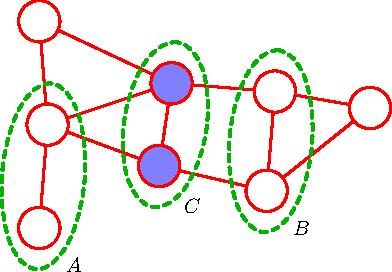
\includegraphics[width=.3\linewidth]{./figures/dep.pdf}
}
\subfigure[Граф с кликами]{
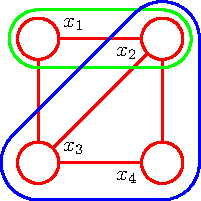
\includegraphics[width=.3\linewidth]{./figures/clique.pdf}
}\label{fig:mrf}
\caption{Примеры}
\end{figure}


\section{Примеры}

В качестве примеров рассмотрим модель Потта. Совместное распределение имеет вид \eqref{eqn:eng_function} с  функцией энергии равной
\begin{equation}
U(x) = -\sum\limits_{i\sim j} J_{ij}\delta(x_i, x_j) - \sum\limits_i H_i x_i.
\end{equation}
Тут $i \sim j$ означает, что (i, j) $\in \mathcal{E}$, $\delta$ -- дельта Кронекера, а матрица $J$ и вектор $H$ являются параметрами модели.
При этом, случайные величины имеют некоторое дискретное распределение на множестве $A = \{a_1, \ldots, a_k\}$. Если $k = 2$, $A = \{ 1, -1\}$  и  функция энергии имеет вид
\begin{equation}
U(x) = -J\sum\limits_{i\sim j} \delta(x_i, x_j) - H\sum\limits_i  x_i,
\end{equation}
то такая модель называется моделью Изинга.

Обозначим 
\begin{gather*}
f(y \mid \theta) = q_{\theta}(y)/Z_{\theta}, \ \ Z_{\theta} = \sum\limits_{y} q_{\theta}(y) 
\end{gather*}

В таких моделях константа $Z$ не может быть точно вычислена для больших графов. Поэтому  максимизация функционала правдоподобия и вычисление апостериорного распределения
\begin{gather*}
\pi(\theta \mid y) = q_\theta(y)\pi_0(\theta)/Z_{\theta},
\end{gather*}
при заданном априорном $\pi_0(\theta)$ также затруднительно в связи с неизвестной $Z_\theta$.

Стандартным методом при работе с Байесовскими оценками является метод марковских цепей Монте-Карло (тут подробнее расписать алгоритм Метрополиса-Гастингса).
Но для этого необходимо уметь считать следующую доверительную вероятность
\begin{equation}
H(\theta'\mid \theta) = \frac{q_{\theta'}(y) \pi_0(\theta')Z_{\theta} p(\theta\mid\theta')}{q_{\theta}(y) \pi_0(\theta)Z_{\theta'} p(\theta'\mid\theta)},
\end{equation}
то есть вычислять $Z_{\theta}/Z_{\theta'}$.



Один из вариантов оценить нормализующую константу как
\begin{gather*}
\widehat{Z}_{\theta} = \frac{1}{B} \sum\limits_{t=1}^B \frac{q_\theta(x^{(t)})}{g(x^{(t)})}, \ \  \text{где} \ x^{(1)}, \ldots, x^{(B)} \sim g.
\end{gather*}
Для некоторой плотности $g(x)$, носитель которой содержит носитель $q_{\theta}$. Дисперсия такой оценки зависит от $q_\theta/g$ и поэтому нужно выбирать $g$ максимально близко к $q_\theta$. Например, можно выбрать $g = f(x \mid \theta')$ для некоторого $\tilde{\theta}$ (то есть из того же самого семейства распределений).

	

% Существует несколько задач, связанных с MRF 
% \begin{enumerate}
% \item Оценка параметров совместного распределения (в предположении, что известна структура графа)
% \item Оценка структуры графа
% \item Определение вероятности данной конфигурации графа (выборки)
% \item Определение наиболее вероятной конфигурации при условии некоторой информации
% \end{enumerate}
% Обычно первая задача решается оптимизацией функционала правдоподобия.

% Рассмотрим последнюю задачу на примере очисти изображения от шума.

% \section{Пример 1}
% Рассмотрим граф со структурой, представленной на рисунке \ref{fig:example}.
% Пусть каждая вершина $Y_i$ представляет собой пиксель от 0 до 255.
% Рассмотрим зашумленное изображение 
% \begin{gather*}
% Y_i = X_i + e_i, 
% \end{gather*}
% где $e_i \sim \mathcal{N}(0, \sigma^2)$.
% Тогда стоит задача найти 
% \begin{gather*}
% arg\max\limits_X P(X \mid Y).
% \end{gather*}

% По формуле условной вероятности (тут $X = X_\mathcal{N}$)
% \begin{gather*}
% P(X\mid Y) = \frac{P(Y\mid X)P(X)}{P(Y)}.
% \end{gather*}
% Учитывая, что $P(Y_i\mid X_i) =  P(Y_i\mid X)$ и что $Y_i$ независимы, при условии, что все элементы $X$ фиксированы, получаем
% \begin{gather*}
% P(X\mid Y) = \frac{\prod P(Y_i\mid X_i)P(X)}{P(Y)}.
% \end{gather*}

% При этом 
% \begin{gather*}
% P(Y_i\mid X_i) = \frac{1}{\sqrt{2\pi\sigma^2}} \exp(\frac{(Y_i - X_i)}{2\sigma^2}).
% \end{gather*}
% Таким образом, 
% \begin{gather*}
% V_C(X_i) = \frac{(Y_i - X_i)^2}{2\sigma^2}.
% \end{gather*}

\end{document}